\chapter{LAN and WLAN}

\section{Home Preparation}

\begin{center}
\sffamily\small
\begin{tabular}{>{\columncolor{tablegray}}p{15cm}}
\multicolumn{1}{>{\columncolor{tablered}}l}{Important}\\
For this practical exercise, you have to submit a report the answers to the questions below. When submitting the answers to the questions, be brief but precise. If you include screenshots, indicate on the screenshot what is the answer.\\
\hline
\end{tabular}
\end{center}

Connect to the web configuration interface of your home access point.

\begin{center}
\sffamily\small
\begin{tabular}{>{\columncolor{tablegray}}p{15cm}}
\multicolumn{1}{>{\columncolor{tableorange}}l}{Questions \textbf{(3 $\times$ 1.5\,\%)}}\\
What are the range of frequency channels available for your access point?\\
\hline
What are the physical layer data rates supported by your access point?\\
\hline
What are the security protocols supported by your access point?\\
\hline
\end{tabular}
\end{center}

Perform a survey and find the information of available wireless networks. On a Windows computer, you can use the following command:

\begin{lstlisting}
netsh wlan show networks mode=bssid
\end{lstlisting}
On a Ubuntu computer, you can use the following command:

\begin{lstlisting}
sudo iwlist <wlan-interface> scan
\end{lstlisting}

\begin{center}
\sffamily\small
\begin{tabular}{>{\columncolor{tablegray}}p{15cm}}
\multicolumn{1}{>{\columncolor{tableorange}}l}{Task \textbf{(5.5\,\%)}}\\
Add the survey to your report, including the following information for each network:
\begin{itemize}
\item the network name (SSID or ESSID)
\item radio type
\item radio channel
\item physical layer data rates
\item security settings
\end{itemize}\\
\hline
\end{tabular}
\end{center}

\section{Equipment}

Each group requires at least \emph{two} (2) or \emph{three} (3) computers. Start one computer in Windows and the other one in Ubuntu. The hardware we shall use during this lab is the \emph{Cisco Aironet 1200} access point. The firmware of the access point is \emph{CISCO IOS Version 12.3(8)JA2}, and you can download the corresponding at the following link:

\url{http://www.jaumebarcelo.info/teaching/lxs/wlan/WLAN_manual.pdf}

To test copying a file across the wireless network, install an FTP server on one of the computers, such as \emph{Filezilla} in Windows and \emph{vsftpd} in Ubuntu. You may use a web browser as an FTP client.

\begin{itemize}

\item On Windows, install and open \emph{Filezilla}, and connect locally from the same PC using the \emph{loopback} interface 127.0.0.1. Create a new user (username \texttt{\color{blue}test} and password \texttt{\color{blue}test}) and share a local folder with several large files. Do not forget to remove the proxy configuration, or select not to use a proxy server for local addresses.

\item On Ubuntu, install \emph{vsftpd} with the following command:
\begin{lstlisting}
sudo apt-get install vsftpd
\end{lstlisting}
    Once installed, you can find and modify the FTP server configuration in the file \texttt{/etc/vsftpd/vsftpd.conf}. If you need to change the configuration, do not forget to restart the FTP server with the command:
\begin{lstlisting}
sudo services vsftpd restart
\end{lstlisting}
    The server allows by default anonymous access, and therefore you do not need to create a new user. The default shared folder is \texttt{/var/ftp}.
\end{itemize}

\section{Disable Your Local Firewall and Pay Attention to Your Browser}

Your local firewall can interfere with the assignment. Disable the firewall on both Windows and Ubuntu computers. On a Ubuntu computer, you can disable it using the following command:

\begin{lstlisting}
sudo ufw disable
\end{lstlisting}

\begin{center}
\sffamily\small
\begin{tabular}{>{\columncolor{tablegray}}p{15cm}}
\multicolumn{1}{>{\columncolor{tablered}}l}{Important}\\
We recommend using \emph{Internet Explorer} to interact with the access point web interface. If you decide to use \emph{Firefox} to connect to the access point during the assignment, it might be necessary to disable the proxy settings and to uncheck the \emph{offline navigation} option.\\
\hline
\end{tabular}
\end{center}

\section{Basic LAN Configuration}

Connect the Windows and the Ubuntu computers using a cross-over cable, as shown in the figure \ref{fig:Lan}. Configure the interfaces with an IPv4 address if needed. Check layer 2 connectivity using the LED or the \texttt{\color{blue}ethtool} command in Ubuntu. Check layer 3 connectivity and measure round-trip time using \texttt{\color{blue}ping}.

\begin{figure}
\centering
\ifpdf
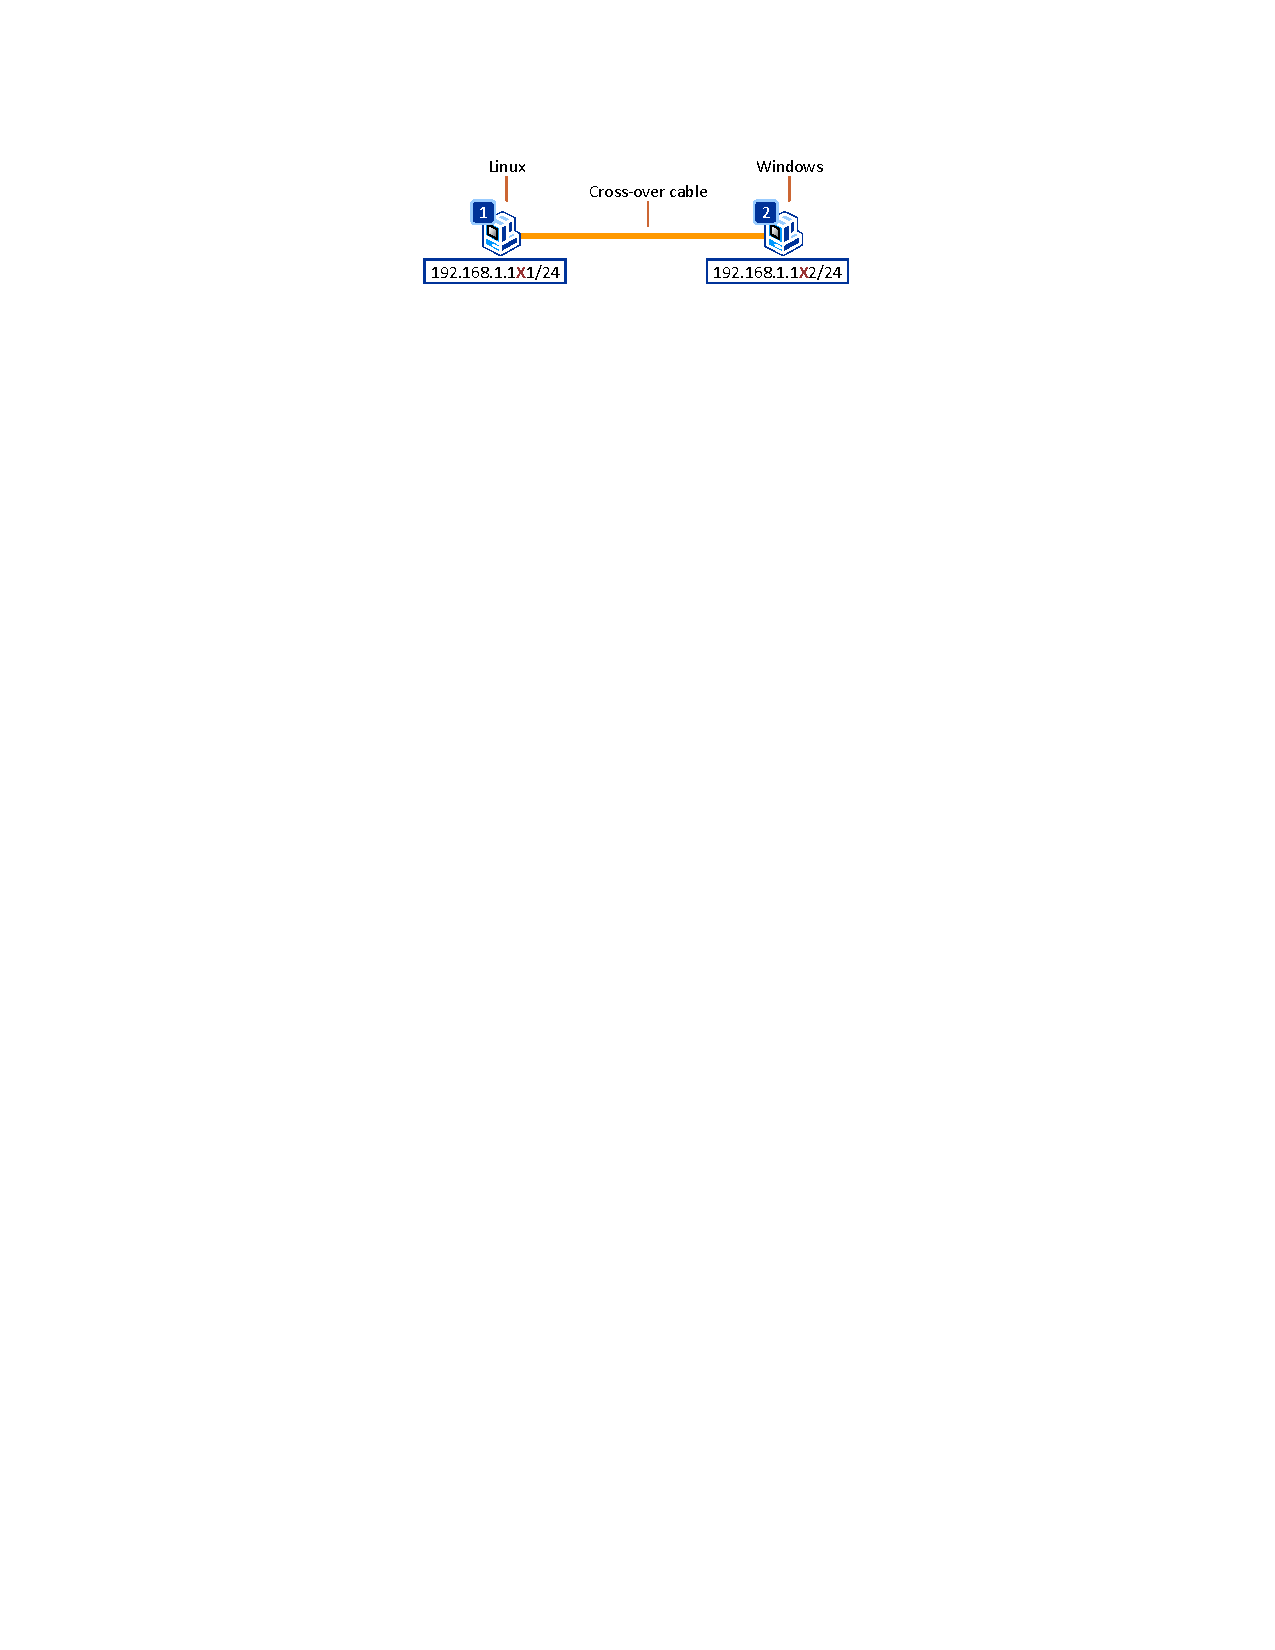
\includegraphics[width=0.9\linewidth]{Figures/Lan.pdf}
\else
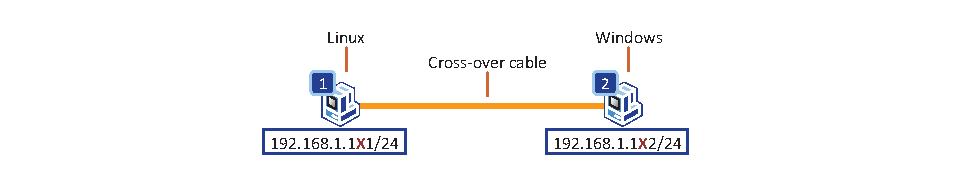
\includegraphics[width=0.9\linewidth]{Figures/Lan.eps}
\fi
\caption{The network topology used for the LAN exercise.}
\label{fig:Lan}
\end{figure}

Next, you need to estimate the available bandwidth using an FTP file transfer or the \texttt{\color{blue}iperf} tool. You must select a file of at least 100\,MB or larger. Change the Ethernet connection speed to 10 Mbps (full duplex) and estimate the bandwidth again.

On a Windows computer use the configuration of you network interface card to change the speed. On a Ubuntu machine, you can check your Ethernet interface configuration using the command:
\begin{lstlisting}
ethtool eth0
\end{lstlisting}

and change the configuration:
\begin{lstlisting}
sudo ethtool -s eth0 speed 10 duplex half
\end{lstlisting}

After testing, remember to change the configuration back:
\begin{lstlisting}
sudo ethtool -s eth0 speed 1000 duplex full
\end{lstlisting}

\begin{center}
\sffamily\small
\begin{tabular}{>{\columncolor{tablegray}}p{15cm}}
\multicolumn{1}{>{\columncolor{tableorange}}l}{Task \textbf{(10\,\%)}}\\
Include a brief report of your activity, which must include the following information:
\begin{itemize}
\item the selected speed for the network interface of each computer
\item the size (in bytes) of the file you transferred using FTP
\item the download duration
\end{itemize}\\
\hline
\end{tabular}
\end{center}

\begin{center}
\sffamily\small
\begin{tabular}{>{\columncolor{tablegray}}p{15cm}}
\multicolumn{1}{>{\columncolor{tableorange}}l}{Questions \textbf{(2 $\times$ 5\,\%)}}\\
What is the average file transfer speed that you obtained for the file download in each instance?\\
\hline
Does the transmission speed reach the physical layer bandwidth? Why do you believe this is so?\\
\hline
\end{tabular}
\end{center}

\section{WLAN Basic Configuration}

WLANs can be used as an access point (AP) to LANs. They can also be used to interconnect to LANs using wireless distribution system (WDS).
WDS can also be used to extend the coverage of a WLAN with access points that do not have a wired connection.
IEEE 802.11 headers can accommodate up to 4 addresses to differentiate between final addresses and per-hop addresses\footnote{This is explained in the theory session}.

Connect the access point to the Windows computer as shown in the figure \ref{fig:Wlan}. You may use either a direct connection or a connection using the patch panel. Use the Internet Explorer browser to connect to the access point web interface. The IP address is available on the access point, and the administrator user is \texttt{\color{blue}Cisco} and the password is \texttt{\color{blue}Cisco}.

\begin{figure}
\centering
\ifpdf
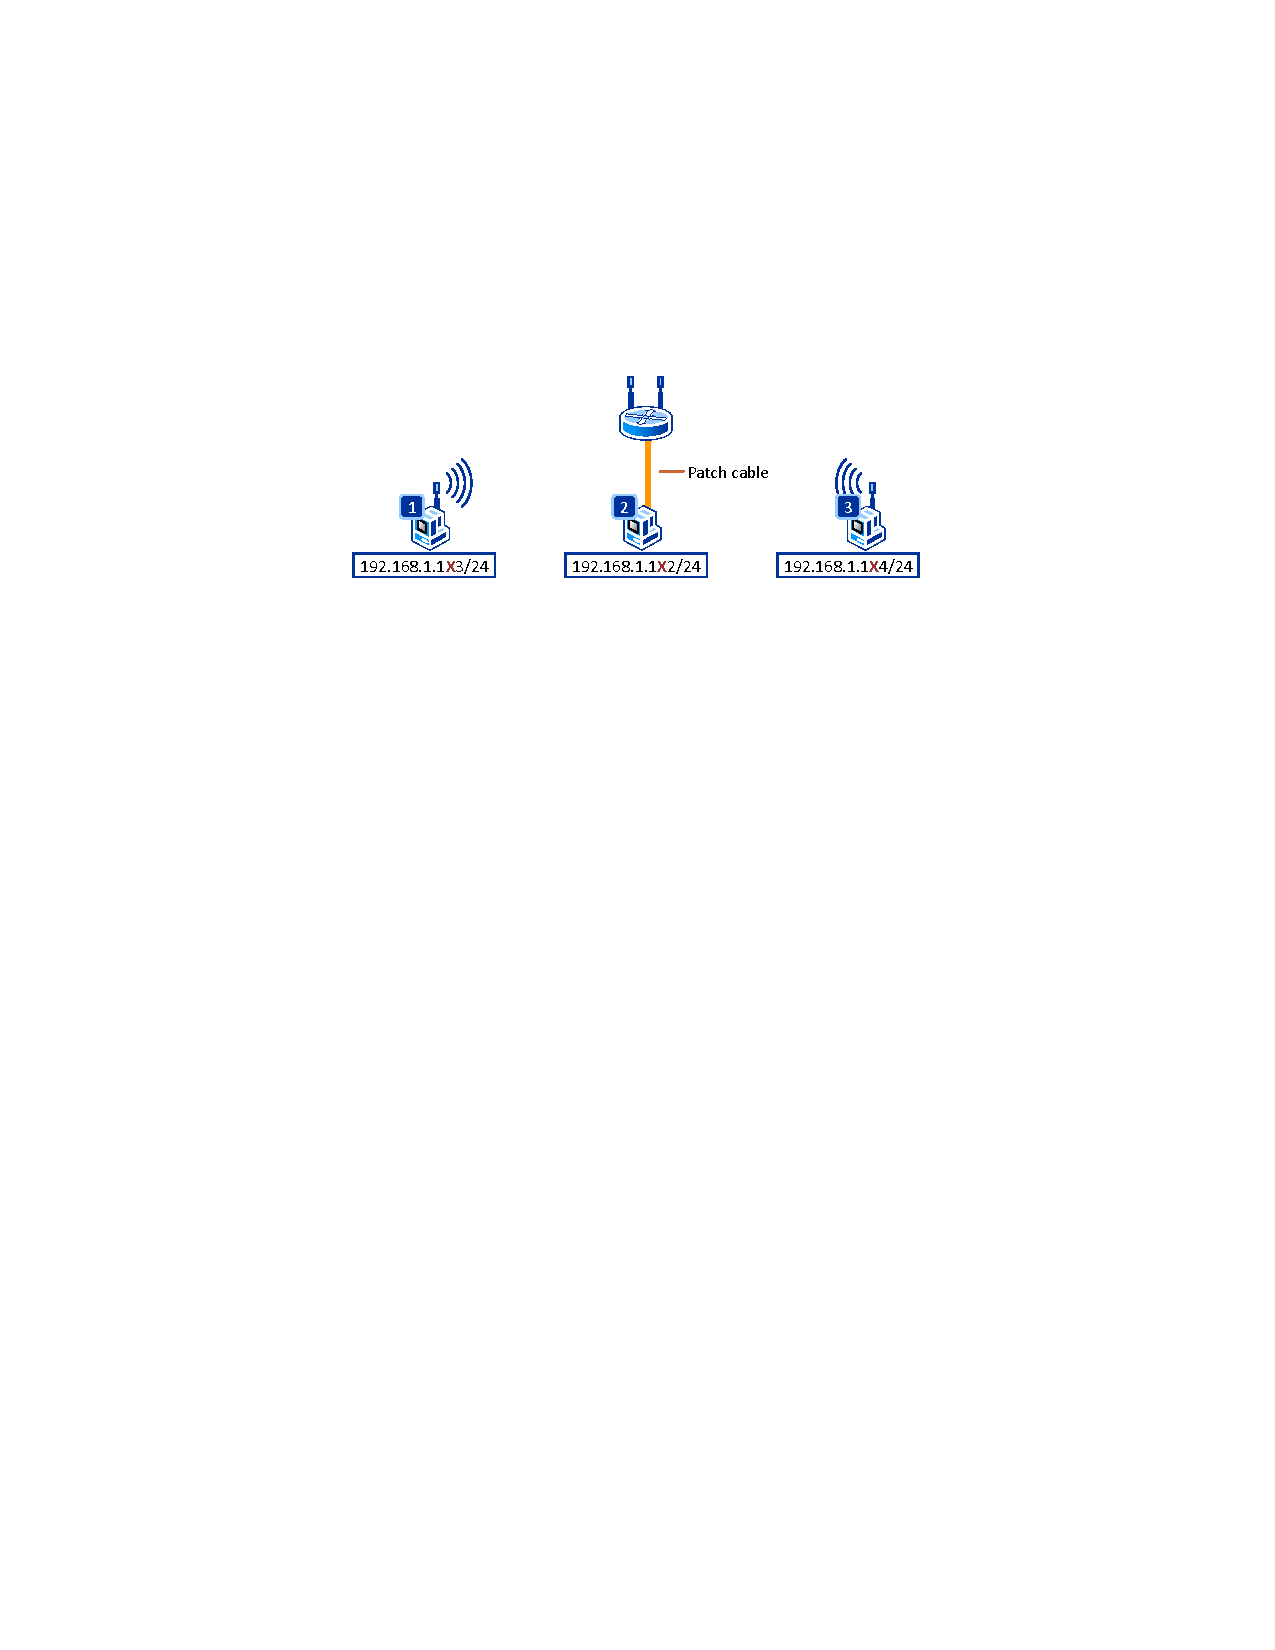
\includegraphics[width=0.9\linewidth]{Figures/Wlan.pdf}
\else
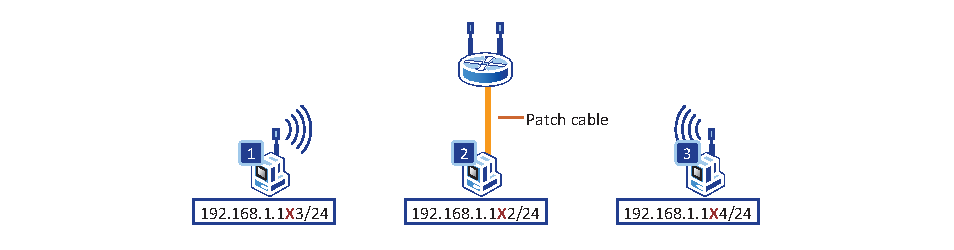
\includegraphics[width=0.9\linewidth]{Figures/Wlan.eps}
\fi
\caption{The network topology used for the WLAN exercise.}
\label{fig:Wlan}
\end{figure}

Go to the \textbf{\sf Express Security} page and configure the access point with the following settings, where \emph{X} is the number of your group.

\begin{center}
\sffamily\small
\begin{tabular}{>{\columncolor{tablegray}}ll}
\multicolumn{1}{>{\columncolor{tableorange}}c}{Setting} & \multicolumn{1}{>{\columncolor{tableheader}}c}{Value}\\
SSID & \texttt{LAB-XIS-{\color{red}X}} \\
\hline
Broadcase SSID in Beacon & Selected \\
\hline
VLAN & No VLAN \\
\hline
Security & No Security \\
\hline
\end{tabular}
\end{center}

Go to the \textbf{\sf Network Interfaces} \textgreater \textbf{\sf Radio0-802.11G} page and enable the radio interface of the access point.

Install a wireless interface in the Ubuntu computer from the previous exercise, and, if available another wireless interface in the third computer. Connect both computers with a wireless interface to the access point that you have just configured. Check that you have network connectivity and use the \texttt{\color{blue}ipconfig} (on Windows) or \texttt{\color{blue}ifconfig} (on Ubuntu) commands to look at the interface configuration. If you have network connectivity, you should be able to ping the other computers of your group (both with wired and wireless connections).

\begin{center}
\sffamily\small
\begin{tabular}{>{\columncolor{tablegray}}p{15cm}}
\multicolumn{1}{>{\columncolor{tableorange}}l}{Tasks \textbf{(3 $\times$ 5\,\%)}}\\
Measure the throughput using FTP to transfer a large file from the wireless computer to the wired one and the other way around.  Include a brief description (a few sentences) of your activity.\\
\hline
Measure the round-trip-time using \texttt{\color{blue}}ping. Include a brief description (a few sentences) of your activity and of the obtained round-trip time.\\
\hline
Use either the \texttt{\color{blue}netsh} or \texttt{\color{blue}iwlist} commands to detect the available wireless networks. Include in your report their configuration.\\
\hline
\end{tabular}
\end{center}

\begin{center}
\sffamily\small
\begin{tabular}{>{\columncolor{tablegray}}p{15cm}}
\multicolumn{1}{>{\columncolor{tableorange}}l}{Questions \textbf{(3 $\times$ 5\,\%)}}\\
Can you reach the physical layer rate maximum throughput? Why do you believe this is so?\\
\hline
Do you observe the same values for the uplink and downlink? \emph{Tip: Perform several experiments in each direction to confirm the measurements.}\\
\hline
If the throughput values for the uplink and downlink differ significantly, why do you believe this is the case?\\
\hline
\end{tabular}
\end{center}

\begin{center}
\sffamily\small
\begin{tabular}{>{\columncolor{tablegray}}p{15cm}}
\multicolumn{1}{>{\columncolor{tablegreen}}l}{Advice}\\
Discuss with the your instructor the interpretation of your results.\\
\hline
\end{tabular}
\end{center}

\section{Hot-Standby}

\begin{center}
\sffamily\small
\begin{tabular}{>{\columncolor{tablegray}}p{15cm}}
\multicolumn{1}{>{\columncolor{tablered}}l}{Important}\\
For this assignment you must collaborate with another group. Ask for the assistance of your instructor before you begin setting up your access point.\\
\hline
\end{tabular}
\end{center}

The hot-standby is a feature to offer high availability. It consists of a backup access point (\emph{AP-standby}) which takes over if the primary AP (\emph{AP-root}) fails. One group will configure the \emph{AP-root} and the other the \emph{AP-standby}. Before you begin disconnect all wireless computers from your access point.

\begin{center}
\sffamily\small
\begin{tabular}{>{\columncolor{tablegray}}p{15cm}}
\multicolumn{1}{>{\columncolor{tablered}}l}{Important}\\
Make sure that you have the same configuration (with the exception of the IP address) on both access points, including the network SSID, network mask and security setting. Ask for the assistance of your instructor if needed.\\
\hline
\end{tabular}
\end{center}

Go to the \textbf{\sf Express Security} page and configure the access point with the following settings, where \emph{X} and \emph{Y} are the numbers of the two groups.

\begin{center}
\sffamily\small
\begin{tabular}{>{\columncolor{tablegray}}ll}
\multicolumn{1}{>{\columncolor{tableorange}}c}{Setting} & \multicolumn{1}{>{\columncolor{tableheader}}c}{Value}\\
SSID & \texttt{LAB-XIS-{\color{red}XY}} \\
\hline
Broadcase SSID in Beacon & Selected \\
\hline
VLAN & No VLAN \\
\hline
Security & No Security \\
\hline
\end{tabular}
\end{center}

\begin{itemize}
\item In the \emph{AP-root}, go to \textbf{\sf Network Interfaces} \textgreater \textbf{\sf Radio 802.11g}, and select \textbf{\sf Access Point (Fallback to radio shutdown)}.
\item In the \emph{AP-standby}, go to \textbf{\sf Services} \textgreater \textbf{\sf Hot Standby}. Select \textbf{\sf Enable} and specify the MAC address that the AP will be monitoring (the radio interface of the root-AP). If the configuration is correct, you should be able to see the status that will appear below on the screen.
\end{itemize}

Connect a wireless computer from each group to the new wireless network that you just configured. Test the wireless connection using the \texttt{\color{blue}ping} command from each wireless computer to the other. If you are using a Windows computer, run the command continuously using the \texttt{\color{blue}-t} switch. 

\begin{center}
\sffamily\small
\begin{tabular}{>{\columncolor{tablegray}}p{15cm}}
\multicolumn{1}{>{\columncolor{tableorange}}l}{Tasks \textbf{(2 $\times$ 4\,\%)}}\\
Draw a sketch of the involved network devices and connections and include it to your report. The sketch must include the MAC and IP addresses of all network interface cards, and of the access point.\\
\hline
Use the \textbf{\sf Home} page of the access points to determine to which access point are the two computers connected. Include a screenshot of this list to your report.\\
\hline
\end{tabular}
\end{center}

Test the standby functionality, by disabling the radio interface of \emph{AP-root} from \textbf{\sf Network Interfaces} \textgreater \textbf{\sf 802.11g} \textgreater \textbf{\sf Settings}. After the time-out expires, the AP-standby should take over with the same SSID and security settings. 

\begin{center}
\sffamily\small
\begin{tabular}{>{\columncolor{tablegray}}p{15cm}}
\multicolumn{1}{>{\columncolor{tableorange}}l}{Tasks \textbf{(2 $\times$ 4\,\%)}}\\
Confirm that the two wireless computers connected to the \emph{AP-standby} by including the output of the \texttt{\color{blue}ping} command and the log from the \textbf{\sf Home} page of the AP configuration interface to your report.\\
\hline
Use the \textbf{\sf Home} page of the access points to determine to which access point are the two computers connected. Include a screenshot of this list to your report.\\
\hline
\end{tabular}
\end{center}

\begin{center}
\sffamily\small
\begin{tabular}{>{\columncolor{tablegray}}p{15cm}}
\multicolumn{1}{>{\columncolor{tableorange}}l}{Questions \textbf{(2 $\times$ 2\,\%)}}\\
How long does it take for the computers to recover the connection after the \emph{AP-root}'s radio is disabled (your best estimate)?\\
\hline
Will the user notice that the connection switches from one AP to the other? How?\\
\hline
\end{tabular}
\end{center}

\section{Configuring an AP as a Repeater}

A repeater AP is not connected to the wired LAN. It is situated within the coverage range of another access point to extend the covered area. Similar to the previous exercise, both access points must share the same configuration (with the exception of the IP address). In this exercise, we shall use the previous \emph{AP-standby} as a repeater.

Before you begin, disconnect your wireless computers from the access point.

\begin{itemize}
\item In the \emph{AP-root}, go to the \textbf{\sf Network Interfaces} \textgreater \textbf{\sf 802.11g} \textgreater \textbf{\sf Settings} page and for the option \textbf{\sf Role in Radio Network} select \textbf{\sf Access Point}.
\item In the \emph{AP-repeater} (the former \emph{AP-standby}) disable the hot-standby option. Go to the \textbf{\sf Security} \textgreater \textbf{\sf SSID Manager} page and at the bottom of the page for the option \textbf{\sf Guest Mode / Set Infrastructure SSID} \textgreater \textbf{\sf Set Single Guest Mode SSID} select the current SSID. In the \textbf{\sf Network Interfaces} \textgreater \textbf{\sf 802.11g} \textgreater \textbf{\sf Settings} page for the option \textbf{\sf Role in Radio Network} choose \textbf{\sf Repeater}.
\end{itemize}

After you have completed the configuration on both access points, connect a wireless computer from each group to the new wireless network that you just configured. Test the wireless connection using the \texttt{\color{blue}ping} command from each wireless computer to the other. If you are using a Windows computer, run the command continuously using the \texttt{\color{blue}-t} switch.

Initially, the client computers are probably connected to the \emph{AP-root}. The \textbf{\sf Home} page from each access point should show the configuration of your network, including the repeater and any connected clients. By selecting the \textbf{\sf Clients} options, you will see the list of associated clients.

\begin{center}
\sffamily\small
\begin{tabular}{>{\columncolor{tablegray}}p{15cm}}
\multicolumn{1}{>{\columncolor{tableorange}}l}{Task \textbf{(6\,\%)}}\\
Include a screenshot of the network configuration from each access point in your report.\\
\hline
\end{tabular}
\end{center}

On the \emph{AP-root}, de-associate a client computer, in which case the client will automatically re-connect to the repeater. After the configuration changes have been completed, your home screen should show the configuration of your network and the repeater, and the clients connected to each AP.

\begin{center}
\sffamily\small
\begin{tabular}{>{\columncolor{tablegray}}p{15cm}}
\multicolumn{1}{>{\columncolor{tableorange}}l}{Tasks \textbf{(2 $\times$ 7\,\%)}}\\
Include a screenshot of the updated network configuration from each access point in your report, after you de-associated a client and the client reconnected to the other access point.\\
\hline
Include the output of the \texttt{\color{blue}ping} command to your report to confirm the the de-associated computer reconnected successfully to the other access point.\\
\hline
\end{tabular}
\end{center}
